\documentclass{uebungszettel}

\usepackage{graphicx}
\usepackage{eurosym}

\usepackage{tikz}
\tikzset{every node/.style={draw, rounded corners, inner sep=0.4cm}}

\begin{document}
\pagestyle{empty}

\maketitle{Klasse 8/9}{10. März 2017}

\begin{aufgabe}{Würfelspiel}
  Maximilian spielt im Kasino folgendes Spiel:

  \begin{addmargin}{1cm}
    Maximilian darf maximal dreimal einen gewöhnlichen Würfel werfen.
    Er kann sich nach jedem Wurf dafür entscheiden, die gewürfelte Augenzahl in Euro ausbezahlt zu bekommen und aufzuhören, oder (falls er noch Würfe übrig hat) neu zu würfeln.
  \end{addmargin}

  Wieviel Gewinn kann Maximilian bei optimaler Spielweise erzielen?
\end{aufgabe}

\begin{aufgabe}{Mensch-Ärgere-Dich-Nicht}
  Rot und Grün spielen miteinander eine Partie.
  Grün ist am Zug, aber Rot kurz vor dem Gewinnen: 
  \begin{center}
    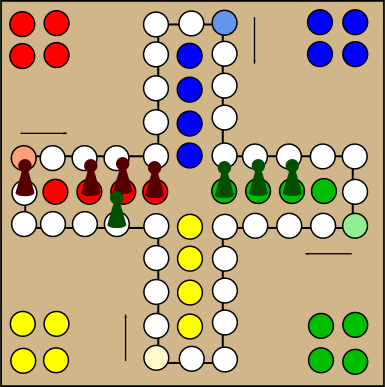
\includegraphics{mensch-aergere-dich-nicht}
  \end{center}
  % Quelle (modifiziert): https://commons.wikimedia.org/wiki/File:Menschenaergern.svg
  \begin{enumerate}
    \item Was ist die Wahrscheinlichkeit, das Rot in einem Zug "`einräumt"', wenn Rot dran ist?
    \item Was ist die Wahrscheinlichkeit, dass die grüne die rote Figur noch schlagen kann, bevor entweder Rot im Haus unterkommt oder Grün vorbeiziehen muss?
  \end{enumerate}
  \begin{center}
    \includegraphics[width=16cm]{mensch-aergere-dich-nicht-zustaende}
  \end{center}
\end{aufgabe}

\begin{aufgabe}{Würfe bis Augenzahl $6$}
  Wie oft musst du durchschnittlich würfeln, bis du eine 6 hast?
\end{aufgabe}

\begin{aufgabe}{Würfe bis zwei Mal Zahl hintereinander}
  Wie oft musst du eine Münze durchschnittlich werfen, bis du zweimal hintereinander Zahl wirfst?
  \begin{center}
    \includegraphics[width=1.25cm]{euro-kopf}
    \includegraphics[width=1.25cm]{euro-kopf}
    \includegraphics[width=1.25cm]{euro-zahl}
    \includegraphics[width=1.25cm]{euro-kopf}
    \includegraphics[width=1.25cm]{euro-zahl}
    \includegraphics[width=1.25cm]{euro-zahl}
  \end{center}
  % Quelle: https://www.ecb.europa.eu/euro/coins/html/de.en.html

  \vspace{1cm}
  \begin{center}
    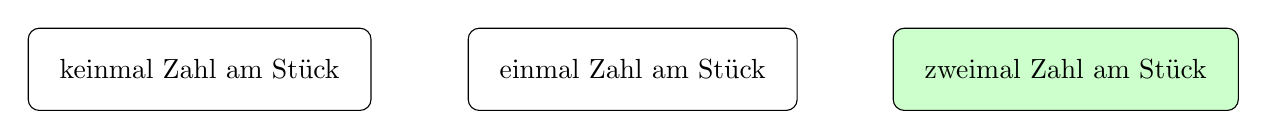
\begin{tikzpicture}
      \node (A) at (-0.5,0) {keinmal Zahl am Stück};
      \node (B) at (5,0) {einmal Zahl am Stück};
      \node [fill=green!20!white] (C) at (10.5,0) {zweimal Zahl am Stück};
    \end{tikzpicture}
  \end{center}
\end{aufgabe}

\begin{aufgabe}{Müsli}
  Jeder Packung Müsli der Firma \textit{Morgenzart} liegt die Figur von einem der drei Musketieren bei.
  Alle drei Figuren sind gleich häufig.
  Wie viele Schachteln Müsli muss ich erwartungsgemäß kaufen, bis ich alle drei Musketiere besitze?

  \vspace{1.5cm}
  \begin{center}
    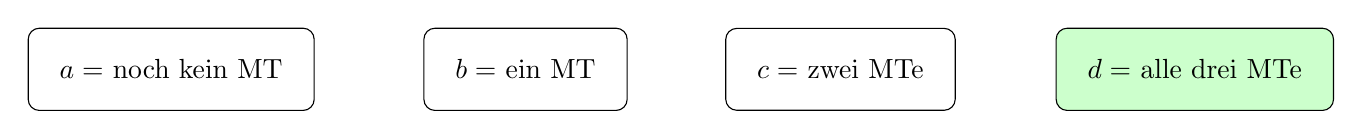
\begin{tikzpicture}
      \node (A) at (-1.5,0) {$a =$ noch kein MT};
      \node (B) at (3,0) {$b =$ ein MT};
      \node (C) at (7,0) {$c =$ zwei MTe};
      \node [fill=green!20!white] (D) at (11.5,0) {$d =$ alle drei MTe};
    \end{tikzpicture}
  \end{center}
  \vspace{1cm}
\end{aufgabe}

\begin{aufgabe}{Die Spinne und die Ameise}
  \begin{minipage}{12cm}
    Ein Marienkäfer und eine Spinne sitzen auf gegenüberliegenden Ecken eines Würfels (siehe Bild).
    Die Spinne entscheidet sich in jedem Zeitschritt zufällig für eine der drei Kanten, die von der Ecke, an der sie sich momentan befindet, wegführen, und läuft diese Kante zur nächsten Ecke.
    Der Marienkäfer ist gelähmt von Angst und bewegt sich nicht.
    Wie lange dauert es erwartungsgemäß, bis die Spinne den Marienkäfer erreicht?
  \end{minipage}
  \hfill
  \begin{minipage}{4cm}
    \includegraphics[width=3.5cm]{spider-and-ladybug}
    % Bildquellen:
    %   Spinne: http://thecraftchop.com/entries/svg/spider-1-2
    %   Marienkäfer: ???
  \end{minipage}

  \vspace{1.5cm}
  \begin{center}
    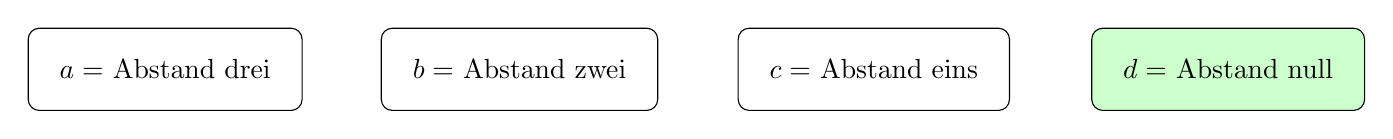
\begin{tikzpicture}
      \node (A) at (0,0) {$a =$ Abstand drei};
      \node (B) at (4.5,0) {$b =$ Abstand zwei};
      \node (C) at (9,0) {$c =$ Abstand eins};
      \node [fill=green!20!white] (D) at (13.5,0) {$d =$ Abstand null};
    \end{tikzpicture}
  \end{center}
  \vspace{1cm}
\end{aufgabe}

\newpage

\begin{aufgabe}{Pistolentriell}
  Drei Banditen $A$, $B$ und $C$ liefern sich in der Wüste ein Pistolenduell auf Leben und Tod.
  Die Regeln sind wie folgt:

  \begin{addmargin}{1cm}
    Solange noch alle drei Banditen am Leben sind, zielt zuerst $A$ auf~$B$, dann $B$ auf~$C$, dann $C$ auf $A$.
    Treffen alle drei nicht, so startet eine neue Runde.
    Wird ein Bandit durch einen anderen erledigt, so beginnt ein Duell zwischen den beiden Überlebenden, wobei der dritte Bandit zuerst auf den eben erfolgreichen Schützen zielt.
    Wird zum Beispiel $B$ von $A$ getroffen, so darf als nächstes $C$ auf $A$ schießen.
  \end{addmargin}

  Die beiden Banditen~$A$ und~$B$ sind mäßig gute Schützen und treffen mit einer Wahrscheinlichkeit von 50\%.
  Dagegen trifft $C$ mit einer Wahrscheinlichkeit von~$75\%$.
  \begin{enumerate}
    \item[a)] Was ist die Wahrscheinlichkeit, dass $A$ überlebt?
    \item[b)] Wie viele Schüsse werden beim Duell erwartungsgemäß abgefeuert?
  \end{enumerate}

  \vspace{1cm}
  \begin{center}
    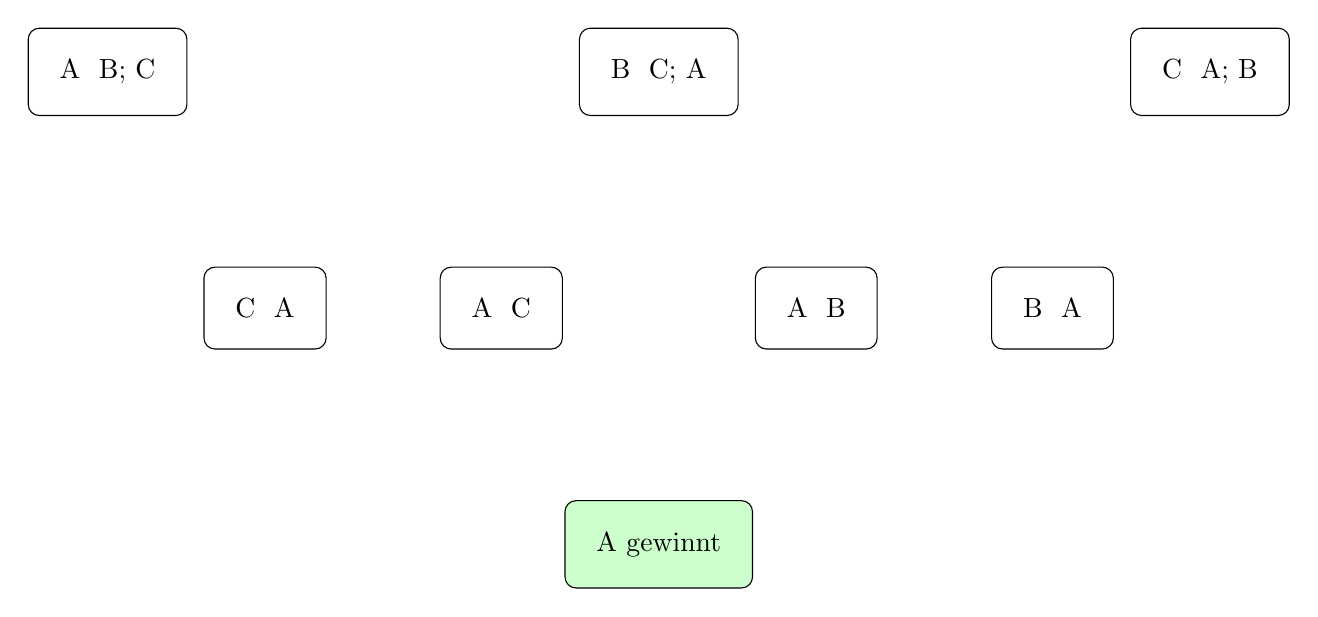
\begin{tikzpicture}
      \node (ABC) at (0,0) {A $\rightarrowtail$ B; C};
      \node (BCA) at (7,0) {B $\rightarrowtail$ C; A};
      \node (CAB) at (14,0) {C $\rightarrowtail$ A; B};
      \node (CA) at (2,-3) {C $\rightarrowtail$ A};
      \node (AC) at (5,-3) {A $\rightarrowtail$ C};
      \node (AB) at (9,-3) {A $\rightarrowtail$ B};
      \node (BA) at (12,-3) {B $\rightarrowtail$ A};
      \node [fill=green!20!white] (Agew) at (7,-6) {A gewinnt};
    \end{tikzpicture}
  \end{center}
\end{aufgabe}

\begin{aufgabe}{Unendlicher Automat ($\star \star \star$)}
  Eine Lotterie bietet einen Automaten zum Verkauf an:
  \begin{addmargin}{1cm}
    Dieser Automat bietet dir einen zufälligen Geldbetrag zwischen 0\euro{} und 100\euro{} an.
    Dabei ist jeder Betrag gleich wahrscheinlich.
    Du kannst diesen Betrag annehmen oder ablehnen.
    Wenn du den Betrag annimmst, so kannst du den Automaten danach nicht mehr benutzen.
    Falls du den Betrag ablehnst, so schaltet sich der Automat für zwei Monate aus.
  \end{addmargin}
  Da du ungeduldig ist, hättest du das Geld lieber heute als in ein paar Monaten.
  Deshalb sind dir $x$\euro{} in zwei Monaten genau so viel wert wie $0,9 \cdot x$\euro{} heute.
  (Du würdest also 9,01\euro{} heute lieber nehmen als 10\euro{} in zwei Monaten.)
  Wie viel würdest du maximal zahlen, um solch einen Automaten zu kaufen?

  {\footnotesize Tipp:
    Sei $x$ der erwartete Nutzen des Automaten, ausgedrückt in Euro, die du heute bekommst.
    (Das heißt, du würdest maximal $x$\euro{} für den Automaten zahlen.)
    Dann ist deine optimale Strategie, das Angebot $y$ des Automaten anzunehmen, falls $y \geq 0,9 \cdot x$ und abzulehnen, falls $y < 0,9 \cdot x$.
    Denn: Im letzten Fall kannst du einen größeren Nutzen erzielen, indem du den Automaten in zwei Monaten benutzt.
    Analysiere, wie häufig die beiden Fälle eintreten und welchen Nutzen du jeweils hast!
   }
\end{aufgabe}

\newpage

\begin{aufgabe}{Galton-Watson-Modelle}
  Wissenschaftler halten eine Kultur von Bakterien in einer Petrischale.
  Jedes Bakterium stirbt mit einer Wahrscheinlichkeit von $\tfrac{1}{4}$ und teilt sich mit einer Wahrscheinlichkeit von $\tfrac{3}{4}$.
  (Wir gehen davon aus, dass die Überlebenswahrscheinlichkeit von Bakterien unabhängig ist, und alle Ressourcen in unbegrenzten Maße zur Verfügung stehen.)
  \begin{itemize}
    \item[a)] Was ist die Wahrscheinlichkeit, dass die Bakterienkultur irgendwann ausstirbt?
    \item[b)]
      Angenommen, jedes Bakterium stirbt mit einer Wahrscheinlichkeit von 60\% und teilt sich mit einer Wahrscheinlichkeit von 40\%.
      Was ist jetzt die Wahrscheinlichkeit, dass die Population irgendwann ausstirbt?
  \end{itemize}
\end{aufgabe}

\end{document}